\documentclass[a4paper]{article}

\usepackage[T1]{fontenc}
\usepackage[american]{babel}
\usepackage[utf8]{inputenc}
\usepackage{fvextra}
\usepackage[autostyle,english=american]{csquotes}
\MakeOuterQuote{"}
\usepackage[
    maxbibnames=99,
    style=numeric,
    sorting=none,
    alldates=iso,
    seconds=true
]{biblatex}
\addbibresource{bib.bib}
\usepackage[
    pdfusetitle,
    pdfkeywords={Line Generalization,Line Simplification,Wang--Mueller},
    pdfborderstyle={/S/U/W 0} % /S/U/W 1 to enable reasonable decorations
]{hyperref}
\usepackage{enumitem}
\usepackage[toc,page,title]{appendix}
\usepackage{caption}
\usepackage{subcaption}
\usepackage{dcolumn}
\usepackage{gensymb}
\usepackage{units}
\usepackage{varwidth}
\usepackage{tabularx}
\usepackage{float}
\usepackage{numprint}
\usepackage{tikz}
\usetikzlibrary{shapes.geometric,arrows,positioning}
\usepackage{fancyvrb}
\usepackage{layouts}
\usepackage{minted}
%\usepackage{charter}
%\usepackage{setspace}
%\doublespacing

\gdef\VCDescribe{2021-05-08 (revision a627e2097554)}%

\newcommand{\smallAngle}{\frac{\pi}{4}}
\newcommand{\isolationThreshold}{0.50}


\newcommand{\onpage}[1]{\ref{#1} on page~\pageref{#1}}
\newcommand{\titlecite}[1]{\citetitle{#1}\cite{#1}}
\newcommand{\titleciteauthor}[1]{\citetitle{#1} by \citeauthor{#1}\cite{#1}}
\newcommand{\DP}{Douglas \& Peucker}
\newcommand{\VW}{Visvalingam--Whyatt}
\newcommand{\WM}{Wang--M{\"u}ller}
\newcommand{\WnM}{Wang and M{\"u}ller}
\newcommand{\WirM}{Wang ir M{\"u}ller}
% {\WM} algoritmo realizacija kartografinei upių generalizacijai
\newcommand{\MYTITLE}{{\WM} algorithm realization for cartographic line generalization}
\newcommand{\MYTITLENOCAPS}{wang--m{\"u}ller algorithm realization for cartographic line generalization}
\newcommand{\MYAUTHOR}{Motiejus Jakštys}
\newcommand{\inputcode}[2]{\inputminted[fontsize=\small]{#1}{#2}}
\newenvironment{longlisting}{\captionsetup{type=listing}}{}

\title{\MYTITLE}
\author{\MYAUTHOR}
\date{\VCDescribe}

\begin{document}

\begin{titlepage}
    \begin{center}
        
\includegraphics[width=0.2\textwidth]{vu.pdf} \\[4ex]

        \large
        \textbf{\textsc{
            vilnius university \\
            faculty of chemistry and geosciences \\
            department of cartography and geoinformatics
        }} \\[8ex]

        \textbf{\MYAUTHOR} \\[8ex]

        \normalsize
        A Thesis Presented for the Degree of Master in Cartography \\[8ex]

        \LARGE
        \textbf{\textsc{\MYTITLENOCAPS}}

        \vfill

        \normalsize
        Supervisor Dr. Andrius Balčiūnas \\[16ex]

        \VCDescribe
    \end{center}
\end{titlepage}

\begin{abstract}
\label{sec:abstract}

    Currently available line simplification algorithms are rooted in
    mathematics and geometry, and are unfit for bendy map features like rivers
    and coastlines. {\WnM} observed how cartographers simplify these natural
    features and created an algorithm. We implemented this algorithm and
    documented it in great detail. Our implementation makes {\WM} algorithm
    freely available in PostGIS, and this paper explains it.

    \vfill

    Šiuo metu prieinami linijų supaprastinimo algoritmai yra kilę iš
    matematikos ir geometrijos, bei yra netinkami lankstiems geografiniams
    objektams, tokiems kaip upės ir pakrantės. {\WirM} ištyrė, kaip kartografai
    vykdo upių generalizaciją, ir sukūrė algoritmą. Mes realizavome šį
    algoritmą ir išsamiai jį dokumentavome. Mūsų {\WM} realizacija ir
    dokumentacija yra nemokami ir laisvai prieinami naudojant PostGIS
    platformą.

\end{abstract}

\newpage

\tableofcontents

\listoffigures
\listoftables
\listoflistings

\newpage

\section{Introduction}
\label{sec:introduction}

\iffalse
NOTICE: this value should be copied to layer2img.py:TEXTWIDTH, so dimensions
of inline images are reasonable.

Textwidth in cm: {\printinunitsof{cm}\prntlen{\textwidth}}
\fi

When creating small-scale maps, often the detail of the data source is greater
than desired for the map. While many features can be removed or simplified, it
is more tricky with natural features that have many bends, like coastlines,
rivers, or forest boundaries.

To create a small-scale map from a large-scale data source, features need to be
simplified, i.e., detail should be reduced. While performing the
simplification, it is important to retain the "defining" shape of the original
feature. Otherwise, if the simplified feature looks too different from the
original, the result will look unrealistic. Simplification problem for some
objects can often be solved by non-geometric means:

\begin{itemize}
    \item Towns and cities can be filtered by the number of inhabitants.
    \item Roads can be eliminated by the road length, number of lanes, or
        classification of the road (local, regional, international).
\end{itemize}

However, things are not as simple for natural features like rivers or
coastlines. If a river is nearly straight, it should remain such after
simplification. An overly straightened river will look like a canal, and the
other way around --- too curvy would not reflect the natural shape. Conversely,
if the river originally is highly wiggly, the number of bends should be
reduced, but not removed altogether. Natural line simplification problem can be
viewed as a task of finding a delicate balance between two competing goals:

\begin{itemize}
    \item Reduce detail by removing or simplifying "less important" features.
    \item Retain enough detail, so the original is still recognizable.
\end{itemize}

Given the discussed complexities with natural features, a fine line between
under-simplification (leaving object as-is) and over-simplification (making a
straight line) needs to be found. Therein lies the complexity of simplification
algorithms: all have different trade-offs.

The purpose of the thesis is to implement a cartographic line generalization
algorithm on the basis of {\WM} algorithm, using open-source software. Tasks:

\begin{itemize}
    \item Evaluate existing line simplification algorithms.
    \item Identify main river generalization problems, using classical line
        simplification algorithms.
    \item Define the method of the {\WM} technical implementation.
    \item Realize {\WM} algorithm technically, explaining the geometric
        transformations in detail.
    \item Apply the created algorithm for different datasets and compare
        the results with national datasets.
\end{itemize}

Scientific relevance of this work --- the simplification processes (steps)
described by the {\WM} algorithm --- are analyzed in detail, practically
implemented, and the implementation is described. That expands the knowledge of
cartographic theory about the generalization of natural objects' boundaries
after their natural defining properties.

In the original {\WM} article introducing the algorithm, the steps are not
detailed in a way that can be put into practice for specific data; the steps are
specified in this work. Practically, this work makes it possible to use open-source software to perform cartographic line generalization. The developed
specialized cartographic line simplification algorithm can be applied by
cartographers to implement automatic data generalization solutions. Given the
open-source nature of this work, the algorithm implementation can be modified
freely.

\section{Literature Review And Problematic}
\label{sec:literature-review-problematic}

\subsection{Available Algorithms}

This section reviews the classical line simplification algorithms, which,
besides being around for a long time, offer easily accessible implementations,
as well as more modern ones, which only theorize, but do not provide an
implementation.

\subsubsection{{\DP}, {\VW} and Chaikin's}
\label{sec:dp-vw-chaikin}

{\DP}\cite{douglas1973algorithms} and {\VW}\cite{visvalingam1993line} are
"classical" line simplification computer graphics algorithms. They are
relatively simple to implement and require few runtime resources. Both of them
accept a single parameter based on desired scale of the map, which makes them
straightforward to adjust for different scales.

Both algorithms are available in PostGIS, a free-software GIS suite:
\begin{itemize}
    \item {\DP} via
        \href{https://postgis.net/docs/ST_Simplify.html}{PostGIS \textsc{st\_simplify}}.

    \item {\VW} via
        \href{https://postgis.net/docs/ST_SimplifyVW.html}{PostGIS
        \textsc{st\_simplifyvw}}.
\end{itemize}

It may be worthwhile to post-process those through Chaikin's line smoothing
algorithm\cite{chaikin1974algorithm} via
\href{https://postgis.net/docs/ST_ChaikinSmoothing.html}{PostGIS
\textsc{st\_chaikinsmoothing}}.

In generalization examples, we will use two rivers: Šalčia and Visinčia.
These rivers were chosen because they have both large and small bends, and
thus are convenient to analyze for both small- and large-scale generalization.
Figure~\onpage{fig:salvis-25} illustrates the original two rivers without any
simplification.

\begin{figure}[ht]
    \centering
    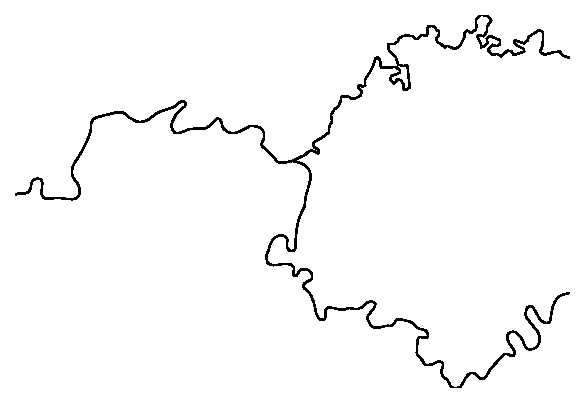
\includegraphics[width=\textwidth]{salvis-25k}
    \caption{Example rivers for visual tests (1:{\numprint{25000}}).}
    \label{fig:salvis-25}
\end{figure}

\begin{figure}[ht]
    \centering
    \begin{subfigure}[b]{.49\textwidth}
        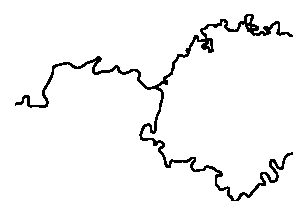
\includegraphics[width=\textwidth]{salvis-50k}
        \caption{Example scaled 1:\numprint{50000}.}
        \label{fig:salvis-50k}
    \end{subfigure}
    \hfill
    \begin{subfigure}[b]{.49\textwidth}
        \centering
        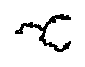
\includegraphics[width=.2\textwidth]{salvis-250k}
        \caption{Example scaled 1:\numprint{250000}.}
    \end{subfigure}
    \caption{Down-scaled original river.}
    \label{fig:salvis-50-250}
\end{figure}

Same rivers, unprocessed but in higher scales (1:\numprint{50000} and
1:\numprint{250000}), are depicted in figure~\ref{fig:salvis-50-250}. Some
river features are so compact that a reasonably thin line depicting the river
is touching itself, creating a thicker line. We can assume that some
simplification for scale 1:\numprint{50000} and especially for
1:\numprint{250000} are worthwhile.

\begin{figure}[ht]
    \centering
    \begin{subfigure}[b]{.49\textwidth}
        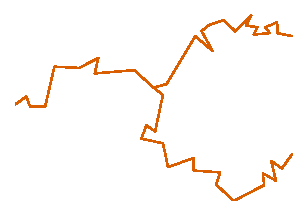
\includegraphics[width=\textwidth]{salvis-douglas-64-50k}
        \caption{Using {\DP}.}
    \end{subfigure}
    \hfill
    \begin{subfigure}[b]{.49\textwidth}
        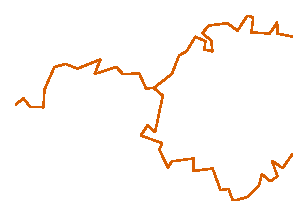
\includegraphics[width=\textwidth]{salvis-visvalingam-64-50k}
        \caption{Using {\VW}.}
    \end{subfigure}
    \caption{Simplified using classical algorithms (1:\numprint{50000}).}
    \label{fig:salvis-generalized-50k}
\end{figure}

Figure~\ref{fig:salvis-generalized-50k} illustrates the same river bend, but
simplified using {\DP} and {\VW} algorithms. The resulting lines are jagged,
and thus the resulting line looks unlike a real river. To smoothen the jaggedness,
traditionally, Chaikin's\cite{chaikin1974algorithm} is applied after
generalization, illustrated in figure~\ref{fig:salvis-generalized-chaikin-50k}.

\begin{figure}[ht!]
    \centering
    \begin{subfigure}[b]{.49\textwidth}
        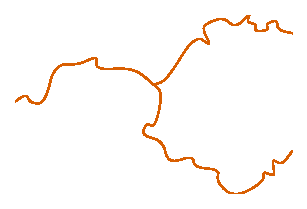
\includegraphics[width=\textwidth]{salvis-douglas-64-chaikin-50k}
        \caption{{\DP} and Chaikin's.}
        \label{fig:salvis-douglas-64-chaikin-50k}
    \end{subfigure}
    \hfill
    \begin{subfigure}[b]{.49\textwidth}
        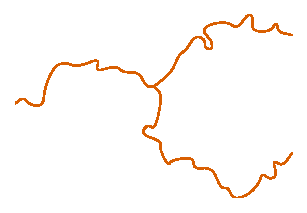
\includegraphics[width=\textwidth]{salvis-visvalingam-64-chaikin-50k}
        \caption{{\VW} and Chaikin's.}
        \label{fig:salvis-visvalingam-64-chaikin-50k}
    \end{subfigure}
    \caption{Simplified and smoothened river (1:\numprint{50000}).}
    \label{fig:salvis-generalized-chaikin-50k}
\end{figure}

\begin{figure}[ht!]
    \centering
    \begin{subfigure}[b]{.49\textwidth}
        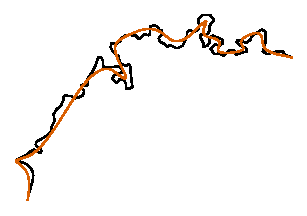
\includegraphics[width=\textwidth]{salvis-overlaid-douglas-64-chaikin-50k}

        \caption{Original (fig.~\ref{fig:salvis-50k}) and simplified
        (fig.~\ref{fig:salvis-douglas-64-chaikin-50k}).}

    \end{subfigure}
    \hfill
    \begin{subfigure}[b]{.49\textwidth}
        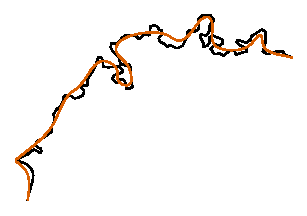
\includegraphics[width=\textwidth]{salvis-overlaid-visvalingam-64-chaikin-50k}

        \caption{Original (fig.~\ref{fig:salvis-50k}) and simplified
            (fig.~\ref{fig:salvis-visvalingam-64-chaikin-50k}.)}

    \end{subfigure}
    \caption{Zoomed-in simplified and smoothened river and original.}
    \label{fig:salvis-overlaid-generalized-chaikin-50k}
\end{figure}

\begin{figure}[b!]
    \centering
    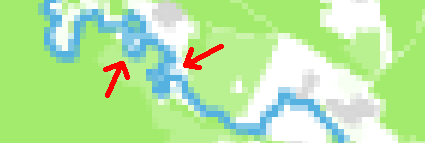
\includegraphics[width=.9\textwidth]{amalgamate1}
    \caption{Narrow bends amalgamating into thick unintelligible blobs.}
    \label{fig:pixel-amalgamation}
\end{figure}

The resulting simplified and smoothened example
(figure~\onpage{fig:salvis-generalized-chaikin-50k}) yields a more
aesthetically pleasing result; however, it obscures natural river features.

Given the absence of rocks, the only natural features that influence the river
direction are topographic:

\begin{itemize}
    \item Relatively straight river (completely straight or with small-angled
        bends over a relatively long distance) implies greater slope, more
        water, and/or faster flow.

    \item Bendy river, on the contrary, implies slower flow, slighter slope,
        and/or less water.

\end{itemize}
Both {\VW} and {\DP} have a tendency to remove the small bends altogether,
removing a valuable characterization of the river.

Sometimes low-water rivers in slender slopes have many bends next to each
other. In low resolutions (either in small-DPI screens or paper, or when the
river is sufficiently zoomed out, or both), the small bends will amalgamate to
a unintelligible blob. Figure~\ref{fig:pixel-amalgamation} illustrates a
real-world example where a bendy river, normally 1 or 2 pixels wide, creates a
wide area, of which the shapes of the bend become unintelligible. In this
example, classical algorithms would remove these bends altogether. A
cartographer would retain a few of those distinctive bends, but would increase
the distance between the bends, remove some of the bends, or both.

% TODO: figues shouldn't split the sentence.

For the reasons discussed in this section, the "classical" {\DP} and {\VW} are
not well-suited for natural river generalization, and a more robust line
generalization algorithm is worthwhile to look for.

\subsubsection{Modern Approaches}

Due to their simplicity and ubiquity, {\DP} and {\VW} have been established as
go-to algorithms for line generalization. During recent years, alternatives
have emerged. These modern replacements fall into roughly two categories:

\begin{itemize}

    \item Cartographic knowledge was encoded to an algorithm (bottom-up
        approach). One among these are \titlecite{wang1998line}, also known
        as {\WM}'s algorithm.

    \item Mathematical shape transformation which yields a more cartographic
        result. E.g., \titlecite{jiang2003line},
        \titlecite{dyken2009simultaneous}, \titlecite{mustafa2006dynamic},
        \titlecite{nollenburg2008morphing}, \titlecite{devangleserrorbends}.

\end{itemize}

Authors of most of the aforementioned articles have implemented the
generalization algorithm, at least to generate the illustrations in the
articles. However, code is not available for evaluation with a desired dataset, much less for use as a basis for creating new maps. To the author's knowledge,
{\WM}\cite{wang1998line} is available in a commercial product, but requires a
purchase of the commercial product suite, without a way to license the
standalone algorithm.

{\WM} algorithm was created by encoding professional cartographers' knowledge
into a computer algorithm. It has a few main properties which make it
especially suitable for generalization of natural linear features:

\begin{figure}[b]
    \centering
    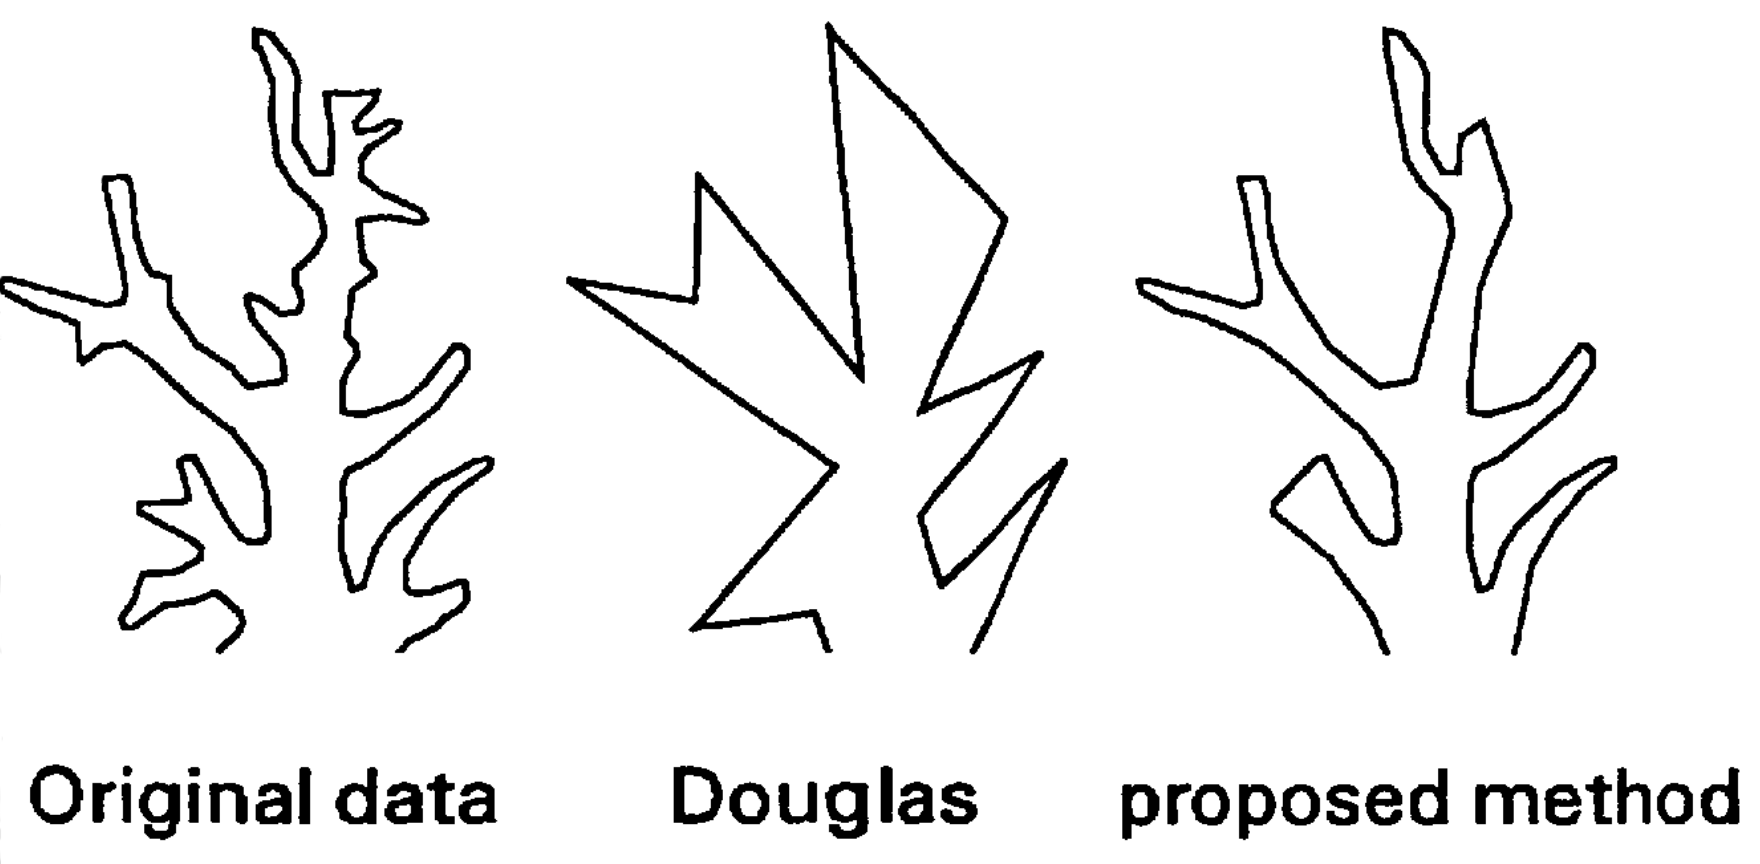
\includegraphics[width=.8\textwidth]{wang125}
    \caption{Figure 12.5 in \cite{wang1998line}: example of cartographic line
    generalization.}
    \label{fig:wang125}
\end{figure}

\begin{itemize}
    \item Small bends are not always removed, but either combined (e.g.,
        3 bends into 2), exaggerated, or removed, depending on the neighboring
        bends.
    \item Long and gentle bends are not straightened, but kept as-is.
\end{itemize}

As a result of these properties, {\WM} algorithm retains the defining
properties of the natural features: high-current rivers keep their appearance
as such, instead of becoming canals; low-stream bendy rivers retain their
frequent small bends.

Figure~\ref{fig:wang125}, sub-figure labeled "proposed method" (from the
original \titlecite{wang1998line}) illustrates the {\WM} algorithm.

\subsection{Problematic with Generalization of Rivers}

This section introduces the reader to simplification and generalization, and
discusses two main problems with current-day automatic cartographic line
generalization:

\begin{itemize}
    \item Currently available line simplification algorithms were created
        to simplify geometries, but do not encode cartographic knowledge.

    \item Existing cartographic line generalization algorithms are not freely
        accessible.
\end{itemize}

\subsubsection{Simplification versus Generalization}

It is important to note the distinction between simplification, line
generalization, and cartographic generalization.

Simplification reduces an object's detail in isolation, not taking the object's
natural properties or surrounding objects into account. For example, if a
river is simplified, it may have an approximate shape of the original river,
but lose some shapes that define it. For example:

\begin{itemize}

  \item Low-water rivers in slender slopes have many small bends next to each
      other. A non-cartographic line simplification may remove all of them,
        thus losing an important river's characteristic feature: after such
        simplification, it will be hard to tell that the original river was
        low-water in a slender slope.

  \item Low-angle river bend river over a long distance differs significantly
      from a completely straight canal. Non-cartographic line simplification
        may replace that bend with a straight line, making the river more
        similar to a canal than a river.

\end{itemize}

In other words, simplification processes the line, ignoring its geographic
features. It works well when the features are human-made (e.g., roads,
administrative boundaries, buildings). There is a number of freely available
non-cartographic line simplification algorithms, which this paper will review.

Contrary to line simplification, cartographic generalization does not focus
into a single feature class (e.g., rivers), but the whole map. For example,
line simplification may change river bends in a way that bridges (and roads to
the bridges) become misplaced. While line simplification is limited to a single
feature class, cartographic generalization is not. Fully automatic cartographic
generalization is not yet a solved problem. % <TODO: Reference needed>.

Cartographic line generalization falls in between the two: it does more than
line simplification, and less than cartographic generalization. Cartographic
line generalization deals with a single feature class, takes into account its
geographic properties, but ignores other features. This paper examines {\WM}'s
\titlecite{wang1998line}, a cartographic line generalization algorithm.

\subsubsection{Availability of Generalization Algorithms}

Lack of robust openly available generalization algorithm implementations poses
a problem for map creation with free software: there is no high-quality
simplification algorithm to create down-scaled maps, so any cartographic work,
which uses line generalization as part of its processing, will be of sub-par
quality. We believe that availability of high-quality open-source tools is an
important foundation for future cartographic experimentation and development,
thus it benefits the cartographic society as a whole.

{\WM}'s commercial availability signals something about the value of the
algorithm: at least the authors of the commercial software suite deemed it
worthwhile to include it. However, not everyone has access to the commercial
software suite, access to funds to buy the commercial suite, or access to the
operating system required to run the commercial suite. PostGIS, in contrast, is
free itself, and runs on free platforms. Therefore, algorithm
implementations that run on PostGIS or other free platforms are useful to a
wider cartographic society than proprietary ones.

\subsubsection{Unfitness of Line Simplification Algorithms}

Section~\ref{sec:dp-vw-chaikin} illustrates the current gaps with line
simplification algorithms for real rivers. To sum up, we highlight the
following cartographic problems from our examples:

\begin{description}

    \item[Long bends] should remain as long bends, instead of becoming fully
        straight lines.

    \item[Many small bends] should not be removed. To retain a river's character,
        the algorithm should retain some small bends, and, when they are too
        small to be visible, they should be combined or exaggerated.

\end{description}

We are limiting the problem to cartographic line generalization. That is, full
cartographic generalization, which takes topology and other feature classes
into account, is out of scope.

Figure~\onpage{fig:wang125} illustrates {\WM} algorithm from their original
paper. Note how the long bends retain curvy, and how some small bends get
exaggerated.

\section{Methodology}
\label{sec:methodology}

The original {\WM}'s algorithm \cite{wang1998line} leaves something to be
desired for a practical implementation: it is not straightforward to implement
the algorithm from the paper alone.

Explanations in this document are meant to expand, rather than substitute, the
original description in {\WM}. Therefore, familiarity with the original paper is
assumed, and, for some sections, having the original close-by is necessary to
meaningfully follow this document.

This paper describes {\WM} in detail that is more useful for anyone who wishes
to follow the algorithm implementation more closely: each section is expanded
with additional commentary, and illustrations added for non-obvious steps. Corner
cases are discussed, too.

Assume Euclidean geometry throughout this document, unless noted otherwise.

\subsection{Main Geometry Elements Used by Algorithm}
\label{sec:vocab}

This section defines and explains the geometry elements that are used
throughout this paper and the implementation.

\begin{description}

    \item[\normalfont\textsc{vertex}] is a point on a plane, can be expressed
        by a pair of $(x,y)$ coordinates.

    \item[\normalfont\textsc{line segment}] or \textsc{segment} joins two
        vertices by a straight line. A segment can be expressed by two
        coordinate pairs: $(x_1, y_1)$ and $(x_2, y_2)$. Line segment and
        segment are used interchangeably.

    \item[\normalfont\textsc{line}] or \textsc{linestring} represents a single
        linear feature. For example, a river or a coastline.

        Geometrically, a line is a series of connected line segments, or,
        equivalently, a series of connected vertices. Each vertex connects to
        two other vertices, with the exception of the vertices at either ends of the line:
        these two connect to a single other vertex.

    \item[\normalfont\textsc{multiline}] or \textsc{multilinestring} is a
        collection of linear features. Throughout this implementation, this is
        used rarely (normally, a river is a single line) but can be valid
        when, for example, a river has an island.

    \item[\normalfont\textsc{bend}] is a subset of a line that humans perceive
        as a curve. The geometric definition is complex and is discussed in
        section~\ref{sec:definition-of-a-bend}.

    \item[\normalfont\textsc{baseline}] is a line between the bend's first and last
        vertices.

    \item[\normalfont\textsc{sum of inner angles}] is a measure of how "curved"
        the bend is. Assume that first and last bend vertices are vectors. Then sum
        of inner angles will be the angular difference of those two vectors.

    \item[\normalfont\textsc{algorithmic complexity}] measured in \textsc{big o
        notation}, is a relative measure that helps explain how
        long\footnote{the upper bound, i.e., the worst case.} the
        algorithm will run depending on its input. It is widely used in computing
        science when discussing the efficiency of a given algorithm.

        For example, given $n$ objects and time complexity of $O(log(n))$, the
        time it takes to execute the algorithm is logarithmic to $n$.
        Conversely, if complexity is $O(n^2)$, then the time it takes to
        execute the algorithm grows quadratically with input. Importantly, if
        the input size doubles, the time it takes to run the algorithm
        quadruples.

        \textsc{big o notation} was first suggested by
        Bachmann\cite{bachmann1894analytische} and Landau\cite{landau1911} in
        late \textsc{xix} century, and clarified and popularized for computing
        science by Donald Knuth\cite{knuth1976big} in the 1970s.

\end{description}

\subsection{Algorithm Implementation Process}
\label{sec:algorithm-implementation-process}

\tikzset{
  startstop/.style={trapezium,text centered,minimum height=2em,
    trapezium left angle=70,trapezium right angle=110,draw=black,fill=red!20},
  proc/.style={rectangle,minimum height=2em,text centered,draw=black,
    fill=orange!20},
  decision/.style={diamond,minimum height=2em,text centered,aspect=3,
    draw=black,fill=green!20},
  arrow/.style={thick,->,>=stealth},
}

\begin{figure}[!ht]
  \centering
  \begin{tikzpicture}[node distance=1.5cm,auto]
    \node (start) [startstop] {Read \textsc{linestring}};
    \node (detect) [proc,below of=start] {Detect bends};
    \node (inflections) [proc,below of=detect] {Fix gentle inflections};
    \node (selfcrossing) [proc,below of=inflections] {Eliminate self-crossing};
    \node (mutated1) [decision,below of=selfcrossing] {Mutated?};
    \node (bendattrs) [proc,below of=mutated1] {Compute bend attributes};
    \node (exaggeration) [proc,below of=bendattrs] {Exaggeration};
    \node (mutated2) [decision,below of=exaggeration] {Mutated?};
    \node (elimination) [proc,below of=mutated2] {Elimination};
    \node (mutated3) [decision,below of=elimination] {Mutated?};
    \node (stop) [startstop,below of=mutated3] {Stop};

    \coordinate [right of=mutated1,node distance=5cm] (mutated1y) {};
    \coordinate [right of=mutated2,node distance=5cm] (mutated2y) {};
    \coordinate [right of=mutated3,node distance=5cm] (mutated3y) {};

    \draw [arrow] (start) -- (detect);
    \draw [arrow] (detect) -- (inflections);
    \draw [arrow] (inflections) -- (selfcrossing);
    \draw [arrow] (selfcrossing) -- (mutated1);
    \draw [arrow] (mutated1) -| node [near start] {Yes} (mutated1y) |- (detect);
    \draw [arrow] (mutated1) -- node[anchor=west] {No} (bendattrs);
    \draw [arrow] (bendattrs) -- (exaggeration);
    \draw [arrow] (exaggeration) -- (mutated2);
    \draw [arrow] (mutated2) -| node [near start] {Yes} (mutated2y) |- (detect);
    \draw [arrow] (mutated2) -- node[anchor=west] {No} (elimination);
    \draw [arrow] (mutated3) -| node [near start] {Yes} (mutated3y) |- (detect);
    \draw [arrow] (mutated3) -- node[anchor=west] {No} (stop);
    \draw [arrow] (elimination) -- (mutated3);
  \end{tikzpicture}
  \caption{Flow chart of the implementation workflow.}
  \label{fig:flow-chart}
\end{figure}

Figure~\ref{fig:flow-chart} visualizes the algorithm steps for each line.
\textsc{multilinestring} features are split to \textsc{linestring} features and
executed in order.

Judging from {\WM} prototype flow chart (depicted in figure 11 of the original
paper), their approach is iterative for the line: it will process the line in
sequence, doing all steps, before moving on to the next step. We will call this
approach "streaming", because it does not require to have the full line to
process it.

We have taken a different approach: process each step fully for the line,
before moving to the next step. This way provides the following advantages:

\begin{itemize}

    \item For \textsc{eliminate self-crossing} stage, when it finds a bend with
        the right sum of inflection angles, it checks the whole line for
        self-crossings. This is impossible with streaming because it requires
        having the full line in memory. It could be optimized by, for example,
        looking for a fixed number of neighboring bends (say, 10), but that
        would complicate the implementation.

    \item \textsc{fix gentle inflections} is iterating the same line twice from
        opposite directions. That could be re-written to streaming fashion, but
        it complicates the implementation, too.

\end{itemize}
On the other hand, comparing to the {\WM} prototype flow chart, our
implementation uses more memory (because it needs to have the full line before
processing), and some steps are unnecessarily repeated, like re-computing the
bend's attributes during repeated iterations.

\subsection{Technical Implementation}
\label{sec:technical-implementation}

Technical algorithm realization was created in \titlecite{postgis311}. PostGIS
is a PostgreSQL extension for working with spatial data.

PostgreSQL is an open-source relational database, widely used in industry and
academia. PostgreSQL can be interfaced from nearly any programming language;
therefore, solutions written in PostgreSQL (and their extensions) are usable in
many environments. On top of that, PostGIS implements a rich set of
functions\cite{postgisref} for working with geometric and geographic objects.

Due to its wide applicability and rich library of spatial functions, PostGIS is
the implementation language of the {\WM} algorithm. The implementation exposes
the entrypoint function \textsc{st\_simplifywm}:

\begin{minted}[fontsize=\small]{sql}
create function ST_SimplifyWM(
  geom geometry,
  dhalfcircle float,
  intersect_patience integer default 10,
  dbgname text default null
) returns geometry
\end{minted}

This function accepts the following parameters:
\begin{description}

    \item[\normalfont\textsc{geom}] is the input geometry. Either
        \textsc{linestring} or \textsc{multilinestring}.

    \item[\normalfont\textsc{dhalfcircle}] is the diameter of the half-circle.
        Explained in section~\ref{sec:bend-scaling-and-dimensions}.

    \item[\normalfont\textsc{intersect\_patience}] is an optional parameter to
        exaggeration operator, explained in
        section~\ref{sec:exaggeration-operator}.

    \item[\normalfont\textsc{dbgname}] is an optional human-readable name of
        the figure. Explained in section~\ref{sec:debugging}.

\end{description}

The function \textsc{st\_simplifywm} calls into helper functions, which detect,
transform, or remove bends. These helper functions are also defined in the
implementation and are part of the algorithm technical realization. All
supporting functions use spatial manipulation functions provided by PostGIS.

\subsection{Automated Tests}
\label{sec:automated-tests}

As part of the algorithm realization, an automated test suite has been
developed. Shapes to test each function have been hand-crafted, and expected
results have been manually calculated. The test suite executes parts of the
algorithm against a predefined set of geometries, and asserts that the output
matches the resulting hand-calculated geometries.

The full set of test geometries is visualized in figure~\ref{fig:test-figures}.

\begin{figure}[ht]
    \centering
    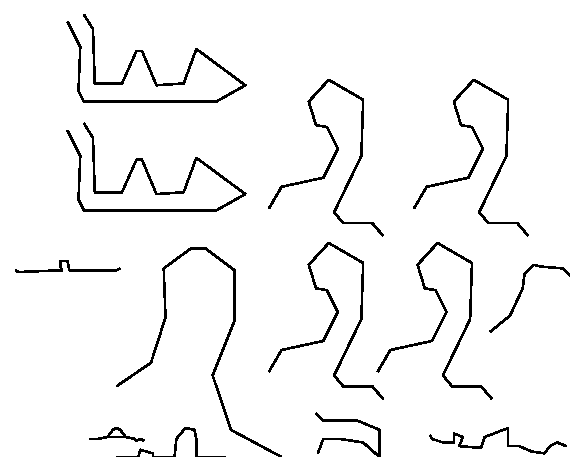
\includegraphics[width=\textwidth]{test-figures}
    \caption{Geometries for automated test cases.}
    \label{fig:test-figures}
\end{figure}

Test suite can be executed with a single command and completes in about a
second. Having an easily accessible test suite boosts confidence that no
unexpected bugs have snug in while modifying the algorithm.

We will explain two instances when automated tests were very useful during
the implementation:
\begin{itemize}

    \item Created a function \textsc{wm\_exaggeration}, which exaggerates bends
        following the rules. It worked well over simple geometries but, due to
        a subtle bug, created a self-crossing bend in Visinčia. The offending
        bend was copied to the automated test suite, which helped fix the bug.
        Now the test suite contains the same bend (a hook-like bend on the
        right-hand side of figure~\ref{fig:test-figures}) and code to verify
        that it was correctly exaggerated.

    \item During algorithm development, automated tests run about once a
        minute. They quickly find logical and syntax errors. In contrast,
        running the algorithm with real rivers takes a few minutes, which
        increases the feedback loop, and takes longer to fix the "simple"
        errors.

\end{itemize}

Whenever we find and fix a bug, we aim to create an automated test case for it,
so the same bug is not re-introduced by whoever works next on the same piece of
code.

Besides testing for specific cases, an automated test suite ensures future
stability and longevity of the implementation itself: when new contributors
start changing code, they have higher assurance they have not broken
already-working code.

\subsection{Reproducibility}
\label{sec:reproducing-the-paper}

It is widely believed that the ability to reproduce the results of a published
study is important to the scientific community. In practice, however, it is
often hard or impossible: research methodologies, as well as algorithms
themselves, are explained in prose, which, due to the nature of the non-machine
language, lends itself to inexact interpretations.

This article, besides explaining the algorithm in prose, includes the program
of the algorithm in a way that can be executed on reader's workstation. On top
of it, all the illustrations in this paper are generated using that algorithm
from a predefined list of test geometries (see
section~\ref{sec:automated-tests}).

This article and accompanying code are accessible on GitHub as of 2021-05-21
\cite{wmsql}.

Instructions how to re-generate all the visualizations are in
appendix~\ref{sec:code-regenerate}. The visualization code serves as a good
example reference for anyone willing to start using the algorithm.

\section{Algorithm Implementation}

Like alluded in section~\ref{sec:introduction}, {\WM} paper skims over
certain details which are important to implement the algorithm. This section
goes through each algorithm stage, illustrating the intermediate steps and
explaining the author's desiderata for a more detailed description.

Illustrations of the following sections are extracted from the automated test
cases which were written during the algorithm implementation (as discussed in
section~\ref{sec:automated-tests}).

\subsection{Debugging}
\label{sec:debugging}

This implementation includes debugging facilities in a form of a table
\textsc{wm\_debug}. The table's schema is written in
listing~\ref{lst:wm-debug-sql}.

\begin{listing}[h]
    \begin{minted}[fontsize=\small]{sql}
drop table if exists wm_debug;
create table wm_debug(
  id serial,
  stage text not null,
  name text not null,
  gen bigint not null,
  nbend bigint,
  way geometry,
  props jsonb
);
    \end{minted}
    \caption{\textsc{wm\_debug} table definition}
    \label{lst:wm-debug-sql}
\end{listing}

When debug mode is active, implementation steps will store their results, which
can be useful to manually inspect the results of intermediate actions. Besides
manual inspection, most of the figure illustrations in this article are
visualized from the \textsc{wm\_debug} table. Debugging mode can be activated
by passing a non-empty \textsc{dbgname} string to the function
\textsc{st\_simplifywm} (this function was described in
section~\ref{sec:technical-implementation}). By convention, \textsc{dbgname} is
the name of the geometry that is being simplified, e.g., \textsc{šalčia}. The
purpose of each column in \textsc{wm\_debug} is described below:

\begin{description}

    \item[\normalfont\textsc{id}] is a unique identifier for each feature.
        Generated automatically by PostgreSQL. Useful when it is necessary to
        copy one or more features to a separate table for unit tests, as
        described in section~\ref{sec:automated-tests}.

    \item[\normalfont\textsc{stage}] is the stage of the algorithm. As of
        writing, there are a few:
        \begin{description}
            \item[\normalfont\textsc{afigures}] at the beginning of the loop.
            \item[\normalfont\textsc{bbends}] after bends are detected.

            \item[\normalfont\textsc{cinflections}] after gentle inflections
                are fixed.

            \item[\normalfont\textsc{dcrossings}] after self-crossings are
                eliminated.

            \item[\normalfont\textsc{ebendattrs}] after bend attributes are
                calculated.

            \item[\normalfont\textsc{gexaggeration}] after bends have been
                exaggerated.

            \item[\normalfont\textsc{helimination}] after bends have been
                eliminated.

        \end{description}

        Some of these have sub-stages which are encoded by a dash and a
        sub-stage name, e.g., \textsc{bbends-polygon} creates polygon
        geometries after polygons have been detected; this particular example
        is used to generate colored polygons in
        figure~\ref{fig:fig8-definition-of-a-bend}.

    \item[\normalfont\textsc{name}] is the name of the geometry, which comes from
        parameter~\textsc{dbgname}.

    \item[\normalfont\textsc{gen}] is the top-level iteration number. In other
        words, the number of times the execution flow passes through
        \textsc{detect bends} phase as depicted in
        figure~\onpage{fig:flow-chart}.

    \item[\normalfont\textsc{nbend}] is the bend's index in its \textsc{line}.

    \item[\normalfont\textsc{way}] is the geometry column.

    \item[\normalfont\textsc{props}] is a free-form JSON object to store
        miscellaneous values. For example, \textsc{ebendattrs} phase stores a
        boolean property \textsc{isolated}, which signifies whether the bend is
        isolated or not (explained in section~\ref{sec:isolated-bend}).

\end{description}

When debug mode is turned off (that is, \textsc{dbgname} is left unspecified),
\textsc{wm\_debug} is empty and the algorithm runs slightly faster.

\subsection{Merging Pieces of the River into One}

Example river geometries were sourced from OpenStreetMap\cite{openstreetmap}
and NŽT\cite{nzt}. Rivers in both data sources are stored in shorter line
segments, and multiple segments (usually hundreds or thousands for significant
rivers) define one full river. While it is convenient to store and edit, these
segments are not explicitly related to each other. This poses a problem for
simplification algorithms which manipulate on full linear features at a time:
full river geometries, but not their parts.

Since these rivers do not have an explicit relationship to connect them
together, they were connected using heuristics: if two line segments share a
name and are within 500 meters from each other, then they form a single river.
For all line simplification algorithms, all rivers need to be combined and
this way proved to be reasonably effective. Source code for this operation can
be found in listing~\onpage{lst:aggregate-rivers.sql}.

\subsection{Bend Scaling And Dimensions}
\label{sec:bend-scaling-and-dimensions}

{\WM} accepts a single input parameter: the diameter of a half-circle. If the
bend's adjusted size (explained in detail in section~\ref{sec:shape-of-a-bend})
is greater than the area of the half-circle, then the bend will be left
untouched. If the bend's adjusted size is smaller than the area of the provided
half-circle, the bend will be simplified: either exaggerated, combined, or
eliminated.

The extent of line simplification, as well as the half-circle's diameter,
depends on the desired target scale. Simplification should be more aggressive
for smaller target scales and less aggressive for larger scales. This section
goes through the process of finding the correct variable to {\WM} algorithm.
What is the minimal, but still eligible, figure that should be displayed on
the map?

According to \titlecite{cartoucheMinimalDimensions}, the map is typically held
at a distance of 30 cm. Recommended minimum symbol size, given viewing distance
of 45 cm (1.5 feet), is 1.5 mm, as analyzed in \titlecite{mappingunits}.

In our case, our target is line bend, rather than a symbol. Assume 1.5 mm is a
diameter of the bend. A semi-circle of 1.5 mm diameter is depicted in
figure~\ref{fig:half-circle}. A bend of this size or larger, when adjusted to
scale, will not be simplified.

\begin{figure}[ht]
  \centering
  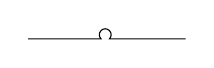
\begin{tikzpicture}[x=1mm,y=1mm]
      \draw[] (-10, 0) -- (-.75,0) arc (225:-45:.75) -- (10, 0);
  \end{tikzpicture}
  \caption{Smallest feature that will be not simplified (to scale).}
  \label{fig:half-circle}
\end{figure}

{\WM} algorithm does not have a notion of scale, but it does have a notion of
distance: it accepts a single parameter $D$, the half-circle's diameter.
Assuming measurement units in projected coordinate system are meters (for
example, \titlecite{epsg3857}), some popular scales are highlighted in
table~\ref{table:scale-halfcirlce-diameter}.

\begin{table}[ht]
    \centering
    \begin{tabular}{ c  D{.}{.}{1} }
        Scale               & \multicolumn{1}{c}{$D(m)$}  \\ \hline
        1:\numprint{10000}  &  15                         \\
        1:\numprint{15000}  &  22.5                       \\
        1:\numprint{25000}  &  37.5                       \\
        1:\numprint{50000}  &  75                         \\
        1:\numprint{250000} & 220                         \\
    \end{tabular}
    \caption{{\WM} half-circle diameter $D$ for popular scales.}
    \label{table:scale-halfcirlce-diameter}
\end{table}


\subsection{Definition of a Bend}
\label{sec:definition-of-a-bend}

The original article describes a bend as:

\begin{displaycquote}{wang1998line}
    A bend can be defined as that part of a line which contains a number of
    subsequent vertices, with the inflection angles on all vertices included in
    the bend being either positive or negative and the inflection of the bend's
    two end vertices being in opposite signs.
\end{displaycquote}

While it gives a good intuitive understanding of what the bend is, this section
provides more technical details. Here are some non-obvious characteristics that
are necessary when writing code to detect the bends:

\begin{itemize}
    \item End segments of each line should also belong to bends. That way, all
        segments belong to 1 or 2 bends.

    \item First and last segments of each bend (except for the two end-line
        segments) are also the first vertex of the next bend.
\end{itemize}

Figure~\ref{fig:fig8-definition-of-a-bend} illustrates the article's figure 8,
but with bends colored as polygons: each color is a distinctive bend.

\begin{figure}[ht]
    \centering
    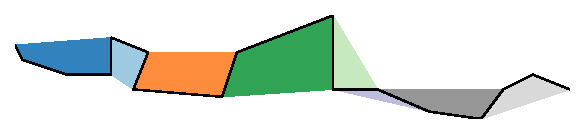
\includegraphics[width=\textwidth]{fig8-definition-of-a-bend}

    \caption{Similar to figure 8 in \cite{wang1998line}: detected bends are
    highlighted.}

    \label{fig:fig8-definition-of-a-bend}
\end{figure}

\subsection{Gentle Inflection at the End of a Bend}

The gist of the section is in the original article:

\begin{displaycquote}{wang1998line}
    But if the inflection that marks the end of a bend is quite small, people
    would not recognize this as the bend point of a bend
\end{displaycquote}

Figure~\ref{fig:fig5-gentle-inflection} visualizes the original paper's figure 5,
when a single vertex is moved outwards the end of the bend.

\begin{figure}[ht]
    \centering
    \begin{subfigure}[b]{.49\textwidth}
        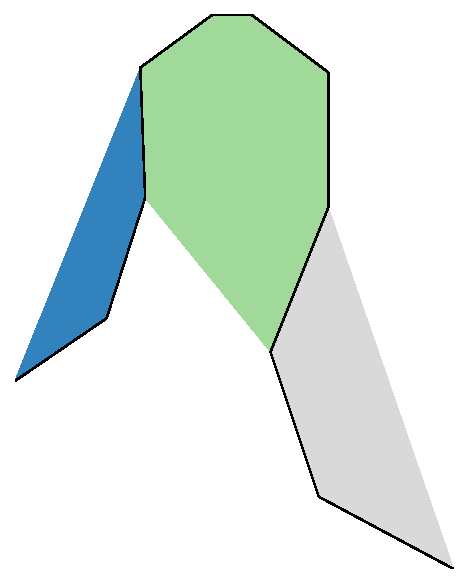
\includegraphics[width=\textwidth]{fig5-gentle-inflection-before}
        \caption{Before applying the inflection rule.}
    \end{subfigure}
    \hfill
    \begin{subfigure}[b]{.49\textwidth}
        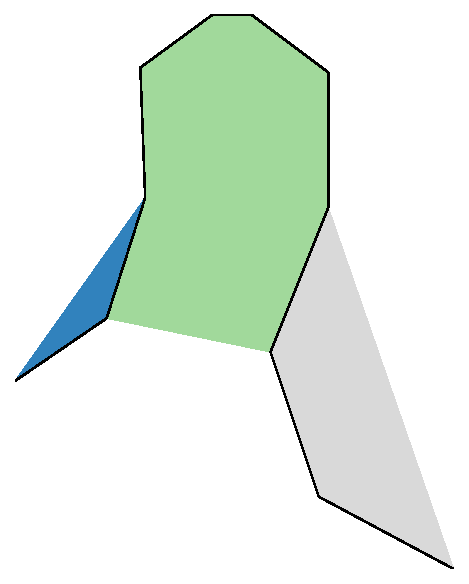
\includegraphics[width=\textwidth]{fig5-gentle-inflection-after}
        \caption{After applying the inflection rule.}
    \end{subfigure}
    \caption{Figure 5 in \cite{wang1998line}: gentle inflections at the ends of
    the bend.}
    \label{fig:fig5-gentle-inflection}
\end{figure}

% TODO: figure should not split the text.

The illustration for this section was clear but insufficient: it does not
specify how many vertices should be included when calculating the end-of-bend
inflection. The iterative approach was chosen: as long as the angle is
"right" and the baseline is becoming shorter, the algorithm should keep
re-assigning vertices to different bends. There is no upper bound
on the number of iterations.

To prove that the algorithm implementation is correct for multiple vertices,
additional example was created and illustrated in
figure~\ref{fig:inflection-1-gentle-inflection}: the rule re-assigns two
vertices to the next bend.

\begin{figure}[ht]
    \centering
    \begin{subfigure}[b]{.49\textwidth}
        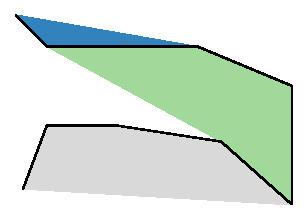
\includegraphics[width=\textwidth]{inflection-1-gentle-inflection-before}
        \caption{Before applying the inflection rule.}
    \end{subfigure}
    \hfill
    \begin{subfigure}[b]{.49\textwidth}
        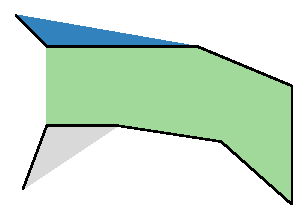
\includegraphics[width=\textwidth]{inflection-1-gentle-inflection-after}
        \caption{After applying the inflection rule.}
    \end{subfigure}
    \caption{Gentle inflection at the end of the bend with multiple vertices.}
    \label{fig:inflection-1-gentle-inflection}
\end{figure}

Note that to find and fix the gentle bends' inflections, the algorithm should
run twice, both ways. Otherwise, if it is executed only one way, the steps will
fail to match some bends that should be adjusted. Current implementation works
as follows:

\begin{enumerate}
    \item Run the algorithm from the beginning to the end.
    \item \label{rev1} Reverse the line and each bend.
    \item Run the algorithm again.
    \item \label{rev2} Reverse the line and each bend.
    \item Return result.
\end{enumerate}

Reversing the line and its bends is straightforward to implement but costly:
the two reversal steps cost additional time and memory. The algorithm could be
made more optimal with a similar version of the algorithm, but the one which
goes backwards. In this case, steps \ref{rev1} and \ref{rev2} could be spared,
that way saving memory and computation time.

The "quite small angle" was arbitrarily chosen to \smallAngle.

\subsection{Self-Line Crossing When Cutting a Bend}

When a bend's baseline crosses another bend, it is called self-crossing.
Self-crossing is undesirable for the upcoming bend manipulation operators; therefore,
should be removed. There are a few rules on when and how they should be removed
--- this section explains them in higher detail, discusses their time
complexity and applied optimizations. Figure~\ref{fig:fig6-selfcrossing} is
copied from the original article.

\begin{figure}[ht]
    \centering
    \includegraphics[width=.5\textwidth]{fig6-selfcrossing}
    \caption{Originally figure 6: the bend's baseline (orange) is crossing a neighboring bend.}
    \label{fig:fig6-selfcrossing}
\end{figure}

\begin{figure}[ht]
    \centering
    \includegraphics[width=.5\textwidth]{selfcrossing-1}
    \caption{The bend's baseline (orange) is crossing a non-neighboring bend.}
    \label{fig:selfcrossing-1-non-neighbor}
\end{figure}

% TODO: figure should not split the text.

Looking at the {\WM} paper alone, it may seem like self-crossing may happen
only with the neighboring bend. This would mean an efficient $O(n)$
implementation\footnote{where $n$ is the number of bends in a line. See
explanation of \textsc{algorithmic complexity} in section~\ref{sec:vocab}.}.
However, as one can see in figure~\ref{fig:selfcrossing-1-non-neighbor}, it may
not be the case: any other bend in the line may be crossing it.

If one translates the requirements to code in a straightforward way, it would
be quite computationally expensive: naively implemented, complexity of checking
every bend with every bend is $O(n^2)$. In other words, the time it takes to
run the algorithm grows quadratically with the number of vertices.

It is possible to optimize this step and skip checking a large number of bends.
Only bends, the inner angles' sum of which is larger than $180^\circ$, can ever
self-cross. That way, only a fraction of bends need to be checked. The
worst-case complexity is still $O(n^2)$, when all bends' inner angles are
larger than $180^\circ$. Having this optimization, the algorithmic complexity
(as a result, the time it takes to execute the algorithm) drops by the
fraction of bends, the inner angles' sum of which is smaller than $180^\circ$.

\subsection{Attributes of a Single Bend}

\textsc{compactness index} is "the ratio of the area of the polygon over the
circle whose circumference length is the same as the length of the
circumference of the polygon" \cite{wang1998line}. Given a bend, its
compactness index is calculated as follows:

\begin{enumerate}

  \item Construct a polygon by joining first and last vertices of the bend.

  \item Calculate the area of the polygon $A_{p}$.

  \item Calculate perimeter $P$ of the polygon. The same value is the
      circumference of the circle: $C = P$.

    \item Given the circle's circumference $C$, the circle's area $A_{c}$ is:

    \[
      A_c = \frac{C^2}{4\pi}
    \]

  \item Compactness index $c$ is the area of the polygon $A_p$ divided by the
      area of the circle $A_c$:

    \[
      c = \frac{A_p}{A_c} =
          \frac{A_p}{ \frac{C^2}{4\pi} } =
          \frac{4\pi A_p}{C^2}
    \]

\end{enumerate}

Once this operation is complete, each bend will have a list of properties
which will be used by other modifying operators.

\subsection{Shape of a Bend}
\label{sec:shape-of-a-bend}

This section introduces \textsc{adjusted size} $A_{adj}$ which trivially
derives from \textsc{compactness index} $c$ and "polygonized" bend's area $A_{p}$:

\[
  A_{adj} = \frac{0.75 A_{p}}{c}
\]

Adjusted size is necessary later to compare bends with each other, or to decide if
the bend is within the simplification threshold.

Sometimes, when working with {\WM}, it is useful to convert between
half-circle's diameter $D$ and adjusted size $A_{adj}$. These easily derive
from circle's area formula $A = 2\pi \frac{D}{2}^2$:

\[
  D = 2\sqrt{\frac{2 A_{adj}}{\pi}}
\]

In reverse, adjusted size $A_{adj}$ from half-circle's diameter:

\[
  A_{adj} = \frac{\pi D^2}{8}
\]

\subsection{Isolated Bend}
\label{sec:isolated-bend}

Bend itself and its "isolation" can be described by \textsc{average curvature},
which is \textcquote{wang1998line}{geometrically defined as the ratio of
inflection over the length of a curve.}

Two conditions must be followed to claim that a bend is isolated:

\begin{enumerate}
    \item \textsc{average curvature} of neighboring bends should be larger
        than the "candidate" bend's curvature. The article did not offer a
        value; this implementation arbitrarily chose $\isolationThreshold$.

    \item Bends on both sides of the "candidate" bend should be longer than a
        certain value. This implementation does not (yet) define such a
        constraint and will only follow the average curvature constraint above.

\end{enumerate}

We believe unclear criteria for \textsc{isolated bend} is one of the main
causes for jagged lines in section~\ref{sec:results}, and is a suggested
further area of research in section~\ref{sec:future-suggestions}.

\subsection{The Context of a Bend: Isolated And Similar Bends}

To find out whether two bends are similar, they are compared by 3 components:

\begin{enumerate}
  \item \textsc{adjusted size} $A_{adj}$.
  \item \textsc{compactness index} $c$.
  \item \textsc{baseline length} $l$.
\end{enumerate}

Components 1, 2 and 3 represent a point in a 3-dimensional space, and Euclidean
distance $d(p,q)$ between those is calculated to differentiate bends $p$ and
$q$:

\[
  d(p,q) = \sqrt{(A_{adj(p)}-A_{adj(q)})^2 +
                   (c_p-c_q)^2 +
                   (l_p-l_q)^2}
\]

The smaller the distance $d$, the more similar the bends are.

\subsection{Elimination Operator}

Figure~\ref{fig:elimination-through-iterations} illustrates steps of figure 8
from the original paper. There is not much to add to the original description
beyond repeating the elimination steps in an illustrated example.

\begin{figure}[ht]
    \centering
    \begin{subfigure}[b]{.7\textwidth}
        \includegraphics[width=\textwidth]{fig8-elimination-gen1}
        \caption{Original}
    \end{subfigure}
    \begin{subfigure}[b]{.7\textwidth}
        \includegraphics[width=\textwidth]{fig8-elimination-gen2}
        \caption{Iteration 1}
    \end{subfigure}
    \begin{subfigure}[b]{.7\textwidth}
        \includegraphics[width=\textwidth]{fig8-elimination-gen3}
        \caption{Iteration 2 (result)}
    \end{subfigure}
    \caption{Originally figure 8: the bend elimination through iterations.}
    \label{fig:elimination-through-iterations}
\end{figure}

\subsection{Combination Operator}
\label{sec:combination-operator}

Combination operator was not implemented in this version.

\subsection{Exaggeration Operator}
\label{sec:exaggeration-operator}

Exaggeration operator finds bends, of which \textsc{adjusted size} is smaller
than the \textsc{diameter of the half-circle}. Once a target bend is found, it
will be exaggerated in increments until either becomes true:

\begin{itemize}
    \item \textsc{adjusted size} of the exaggerated bend is larger than the area of
        the half-circle.

    \item The exaggerated bend starts intersecting with a neighboring bend.
        Then exaggeration aborts, and the bend remains as if it were one step
        before the intersection.

\end{itemize}

Exaggeration operator uses a hardcoded parameter \textsc{exaggeration step} $s
\in (1,2]$. It was arbitrarily picked to {\exaggerationEnthusiasm} for this
implementation. A single exaggeration increment is done as follows:

\begin{enumerate}
    \item Find a candidate bend.
    \item Find the bend's baseline.
    \item Find \textsc{midpoint}, the center of the bend's baseline.

    \item Find \textsc{midbend}, the center of the bend. Distance from one
        baseline vertex to \textsc{midbend} should be the same as from
        \textsc{midbend} to the other baseline vertex.

    \item Mark each bend's vertex with a number between $[1,s]$. The number is
        derived with elements linearly between the start vertex and
        \textsc{midbend}, with values somewhat proportional to the azimuth
        between these lines:

        \begin{itemize}
            \item \textsc{midbend} and the point.
            \item \textsc{midpoint} and the point.
        \end{itemize}

        The other half of the bend, from \textsc{midbend} to the final vertex,
        is linearly interpolated between $[s,1]$, using the same rules as for
        the first half.

        The first version of the algorithm used simple linear interpolation
        based on the point's position in the line. The current version applies
        a few coefficients, which were derived empirically, by observing the
        resulting bend.

    \item Each point (except the beginning and end vertices of the bend) will
        be placed farther away from the baseline. The length of misplacement is
        the marked value in the previous step.

\end{enumerate}

\begin{figure}[ht]
    \centering
    \includegraphics[width=.5\textwidth]{isolated-1-exaggerated}
    \caption{Example isolated exaggerated bend.}
    \label{fig:isolated-1-exaggerated}
\end{figure}

The technical implementation of the algorithm contains two implementations
of exaggeration operator:

\begin{description}

    \item[\normalfont\textsc{wm\_exaggerate\_bend}] is the original one. It
        uses simple linear interpolation. It is fast, but simple. It tends to
        leave jagged bends.

    \item[\normalfont\textsc{wm\_exaggerate\_bend2}] is a more computationally
        expensive function, which leaves better-looking exaggerated bends.

\end{description}

Both functions are inter-change-able and can be found in listing~\ref{lst:wm.sql}.
Figure~\ref{fig:isolated-1-exaggerated} illustrates an exaggerated bend using
\textsc{wm\_exaggerate\_bend2}.

\section{Results}
\label{sec:results}

\subsection{Generalization Results of Analyzed Rivers}
\label{sec:generalization-results-of-analyzed-rivers}

Figures~\ref{fig:salvis-wm-50k} and~\ref{fig:salvis-wm-250k} visualize
the generalization result for Šalčia and Visinčia using {\WM} with the
\textsc{dhalfcircle} values from the
table~\ref{table:scale-halfcirlce-diameter}:

\begin{itemize}
    \item 1:\numprint{50000}: 75.
    \item 1:\numprint{250000}: 220.
\end{itemize}

\subsubsection{Medium-scale (1:\numprint{50000})}
\label{sec:analyzed-medium-scale}

\begin{figure}[ht]
    \centering
    \begin{subfigure}[b]{.49\textwidth}
        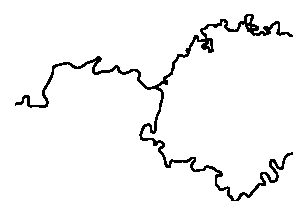
\includegraphics[width=\textwidth]{salvis-50k}
        \caption{Original.}
    \end{subfigure}
    \hfill
    \begin{subfigure}[b]{.49\textwidth}
        \centering
        \includegraphics[width=\textwidth]{salvis-wm-50k}
        \caption{Simplified.}
    \end{subfigure}
    \caption{Simplified with {\WM} for 1:\numprint{50000}.}
    \label{fig:salvis-wm-50k}
\end{figure}

As one can see in figure~\ref{fig:salvis-wm-50k}, the illustrations deliver
what was promised by the algorithm, but with a few caveats. West-side of the
river looks reasonably well simplified: long bends remain slightly curved,
small bends are removed or slightly exaggerated.

Approximately at the middle of the figure some jagged and sharp bends appear.
Figure~\ref{fig:salvis-wm-50k-overlaid-zoom} zooms in, overlaying the original
river (in orange). These will become more pronounced in even larger-scale
simplification in the next section.

\begin{figure}[ht]
    \centering
    \includegraphics[width=\textwidth]{salvis-wm-overlaid-50k-zoom}
    \caption{2x zoomed-in {\WM} for 1:\numprint{50000}.}
    \label{fig:salvis-wm-50k-overlaid-zoom}
\end{figure}

\subsubsection{Large-scale (1:\numprint{250000})}

As visible in figure~\ref{fig:salvis-wm-250k}, for large-scale map, some of the
resulting bends look significantly exaggerated. Why is that?
Figure~\ref{fig:salvis-wm-250k-overlaid-zoom} zooms in the large-scale
simplification and overlays the original (in orange).

\begin{figure}[ht]
    \centering
    \begin{subfigure}[b]{.49\textwidth}
        \centering
        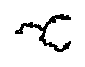
\includegraphics[width=.2\textwidth]{salvis-250k}
        \caption{Original.}
    \end{subfigure}
    \hfill
    \begin{subfigure}[b]{.49\textwidth}
        \centering
        \includegraphics[width=.2\textwidth]{salvis-wm-250k}
        \caption{Simplified.}
    \end{subfigure}
    \caption{Simplified with {\WM} for 1:\numprint{250000}.}
    \label{fig:salvis-wm-250k}
\end{figure}

\begin{figure}[ht]
    \centering
    \includegraphics[width=.8\textwidth]{salvis-wm-overlaid-250k-zoom}
    \caption{10x zoomed-in {\WM} for 1:\numprint{250000}.}
    \label{fig:salvis-wm-250k-overlaid-zoom}
\end{figure}

A conglomeration of bends is visible, especially in north-east side of the
center. We assume this was caused by two bends significantly exaggerated,
leaving no space to exaggerate for those between the two. For the same reason,
the figure~\ref{fig:salvis-wm-50k} (of scale 1:\numprint{50000}) has many
smaller bends at approximately the same location.

\subsection{Comparing Generalized Result with National Spatial Datasets}

\subsubsection{Background}

There are a few datasets used in this comparison: GDB10LT, GDR50LT and
GDR250LT. They are vector datasets, which include rivers. They can be
downloaded for free from \cite{nzt}. Here are the meanings of the codenames:

\begin{description}

    \item[GDB10LT] is dataset of highest detail. Suited for maps of scale
        1:\numprint{10000}.

    \item[GDR50LT] is suited for maps of scale 1:\numprint{50000}.

    \item[GDR250LT] offers least detail, and is suited for maps of
        scale 1:\numprint{250000}.

\end{description}

During the analysis, we ran {\WM} on GDB10LT for 2 destination scales:
1:\numprint{50000} and 1:\numprint{250000}.\footnote{parameter calculation is
detailed in section~\ref{sec:bend-scaling-and-dimensions}.} This section
compares the resulting {\WM}--generalized rivers to GDR50LT and GDR250LT.

\subsubsection{Medium-scale (1:\numprint{50000})}

For our research location, the national dataset GDB10LT is almost equivalent to
GDR50LT. Figure~\ref{fig:salvis-gdr50-overlaid} illustrates it. Therefore, the
comparison between {\WM}--simplified GDB10LT and GDR50LT is equivalent to the
comparison between {\WM}--simplified GDB10LT and non--simplified GDR50LT, which
was covered in section~\ref{sec:analyzed-medium-scale}.

\begin{figure}[ht]
    \centering
    \includegraphics[width=.8\textwidth]{salvis-gdr50-overlaid}
    \caption{GDB10LT (orange) and GDR50LT (black)}
    \label{fig:salvis-gdr50-overlaid}
\end{figure}

\subsubsection{Large-scale (1:\numprint{250000})}

\subsection{Testing Results Online}
\label{sec:testing-results-online}

An on-line tool\cite{openmapwm} has been developed to test incoming parameters
to {\WM} algorithm. A user should select a river of interest, enter the
\textsc{dhalfcircle} parameter and click "Submit". The simplified line feature
will be overlaid on top of the map.

Figure~\ref{fig:openmap-wm-good} illustrates the end result that looks
reasonably well. Figure~\ref{fig:openmap-wm-bad} illustrates that the algorithm
produces poorly simplified results for some geometries.

\begin{figure}[ht]
    \centering
    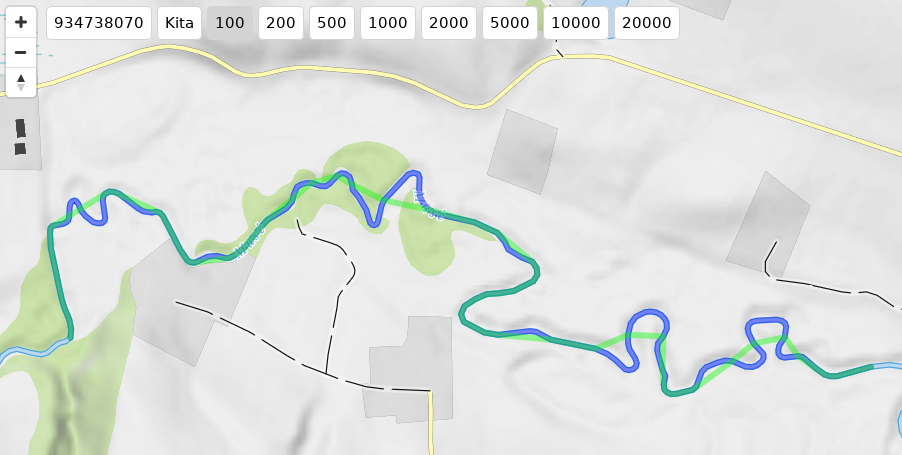
\includegraphics[width=\textwidth]{openmap-wm-good.png}
    \caption{Example on-line test tool for {\WM} algorithm.}
    \label{fig:openmap-wm-good}
\end{figure}

\begin{figure}[ht]
    \centering
    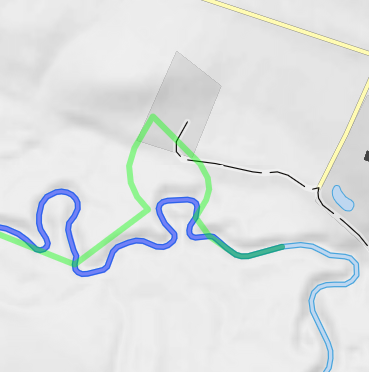
\includegraphics[width=.5\textwidth]{openmap-wm-bad.png}
    \caption{Another example from the on-line test tool.}
    \label{fig:openmap-wm-bad}
\end{figure}

\section{Conclusions}
\label{sec:conclusions}

Classical and modern algorithms line simplification algorithms were evaluated,
main problems with them identified. A method for {\WM} technical
implementation was defined, and the algorithm implemented. Each geometric
transformation was described and visualized. The implemented algorithm was
applied for different shapes and compared to national (Lithuanian) datasets.

About 1,000 lines of Procedural SQL were written for the algorithm and tests,
and a few hundred lines of supporting scripts in Make, Python, Awk, Bash. With
the help of its permissive license and early interest, the algorithm code has
already been used to create a prototype on-line service to evaluate the
algorithm robustness.

\section{Future Suggestions}
\label{sec:future-suggestions}

These are the areas for possible future work with this, published,
implementation:

\begin{itemize}

    \item Implement bend combination operator
        (section~\ref{sec:combination-operator}).

    \item Fine-tune parameters for bend exaggeration.
        Section~\ref{sec:generalization-results-of-analyzed-rivers} contains
        a exaggerated bends that became sharp.

    \item Research when bends should be marked as \textsc{isolated}. As is
        seen from examples, the current criteria is not robust enough.

    \item Once the points above yield a satisfactory result, efficiency of the
        algorithm could be improved to work on the lines in "streaming" fashion
        (more details in section~\ref{sec:algorithm-implementation-process}).

\end{itemize}

That sums up what could be improved without changing the algorithm in a
significant way. Other than that, further area of research is working towards
graduating the algorithm from "isolated cartographic generalization" to "full
cartographic generalization".  The current operators of {\WM} algorithm have a
few venues to preserve the surrounding topology. This could be further
researched and extended.

\section{Acknowledgments}
\label{sec:acknowledgments}

I would like to thank my thesis supervisor, Andrius Balčiūnas, for his help in
formulating the requirements and providing early editorial feedback for the
thesis.

I am grateful to Tomas Straupis, who handed me the {\WM}\cite{wang1998line}
paper on a warm pre-COVID summer evening. I got intrigued. He was also an early
beta-tester of my implementation, and helped me understand where the initial
algorithm descriptions were ambiguous.

Many thanks to NŽT for providing the datasets with a very permissive license.

\printbibliography

\begin{appendices}

\section{Code Listings}

This section contains code listings of the {\WM} algorithm.

\subsection{Re-Generating This Paper}
\label{sec:code-regenerate}

Like explained in section~\ref{sec:reproducing-the-paper}, illustrations in
    this paper are generated from a small list of sample geometries. To observe
    the source geometries or regenerate this paper, run this script (assuming
    the name of this document is \textsc{mj-msc-full.pdf}).

    Listing~\ref{lst:extract-and-generate} will extract the source files from
    the \textsc{mj-msc-full.pdf} to a temporary directory, run the top-level
    \textsc{make} command, and display the generated document. Source code for
    the algorithm, as well as other supporting files, can be found in the
    temporary directory.

\begin{longlisting}
    \inputcode{bash}{extract-and-generate}
    \caption{\textsc{extract-and-generate}}
    \label{lst:extract-and-generate}
\end{longlisting}

\subsection{Function \textsc{st\_simplifywm}}
\begin{longlisting}
    \inputcode{postgresql}{wm.sql}
    \caption{\textsc{wm.sql}}
    \label{lst:wm.sql}
\end{longlisting}

\subsection{Function \textsc{aggregate\_rivers}}
\begin{longlisting}
    \inputcode{postgresql}{aggregate-rivers.sql}
    \caption{\textsc{aggregate-rivers.sql}}
    \label{lst:aggregate-rivers.sql}
\end{longlisting}

\end{appendices}
\end{document}
